\section{Introduction}
\label{sec:introduction}
\note{The importance of gas sensors is made clear. I.e. the need for them in the civil, industrial, medical and military sector. An overview of conventional gas sensors is given. I.e. Bulk-MOX, NDIR, catalytic bead sensor. Novel gas sensors based on 2D structures are presented. Their advantages (small size, flexibility, CMOS-compatibility, sensitivity, specificity) is discussed. Multiple 2D gas sensors are shortly presented. Eventually gas sensors based on 2D TMD heterojunctions are motivated.}

\gibberish{
Gas sensors have been used by humans before the advent of electonic engineering. An prominent example are birds, that accompanied miners in the shafts. If the birds stopped chirping, it was the signal that the oxygen in the air has been replaced by other gases and that the cave should be evacuated as soon as possible. Since then, gas sensors have evolved drastically, and are now mostly free of any animal cruelty. Today gas sensors are not only used for sensing air quality in underground caves, but are also applied in industrial processes, in medical fields , on military battlefields or are used to sense the environment. In the sense of ubiquitous sensing, there is the demand that these sensor become smaller, faster and more power efficient. Trends in that direction allow the development of more efficient industrial processes, increase the efficiency of the medical care or allow precise warnings on the battle field.
There are a variety of types of gas sensors, whose measurement principles range from optical sensing to chemical effects. One of the most popular gas sensor is the carbonmonoxide (CO) sensor, which in many countries is nowadays mandatory to be installed in households. The most common version of this sensor is based on a fuel cell like reaction, which generates an electrical current. This current is highly proportional to the CO concentration in the air. This sensor allows detection of conenctrations as low as XXX ppm. Harmful doses begin at YYY ppm.
Another sensor principle relies on the adsorption of the analyte on the surface of a metal oxide bulk structure. The analyte then exchanges electrons  with the bulk and modulates its conductivity. This effect serves as metric for the concentration of the analyte in the vicinity of the sensor. The sensor can be made quite small, however it has to heated up to around 400 degrees, so that the adsorption effect takes place. The Taguchi sensor is quite popular and its use is very widespread. The Taguchi sensor is sensitive to the gas XXX and can sense concentrations as low as YYY:
Another sensor principle is the NDIR. The sensor analyzes the spectrum of light, that has been transmitted through the analyte. As most gases have a very specific transmittivity spectrum, and the light spectrum of the source is known, the type and concentration of the analyte gas can be determined. This sensor has the major advantage, that it is able to detect various different gases, where as other sensors are only sensitive to single types of gases. However, the sensor requires long intereferomter lengths, and is therefore quite bulky. Such sensor come with a sensitity of XXX (for instance for the gas kryptonitonium).
Currently NDIR sensors are used the most, because of their nice behaviour. Taguchi snesor and MOX sensor fall behind, because they are rather expensive. A detailed overview over the gas sensor market can be seen in \Cref{fig:gas_sensor_market} 
\begin{figure}
    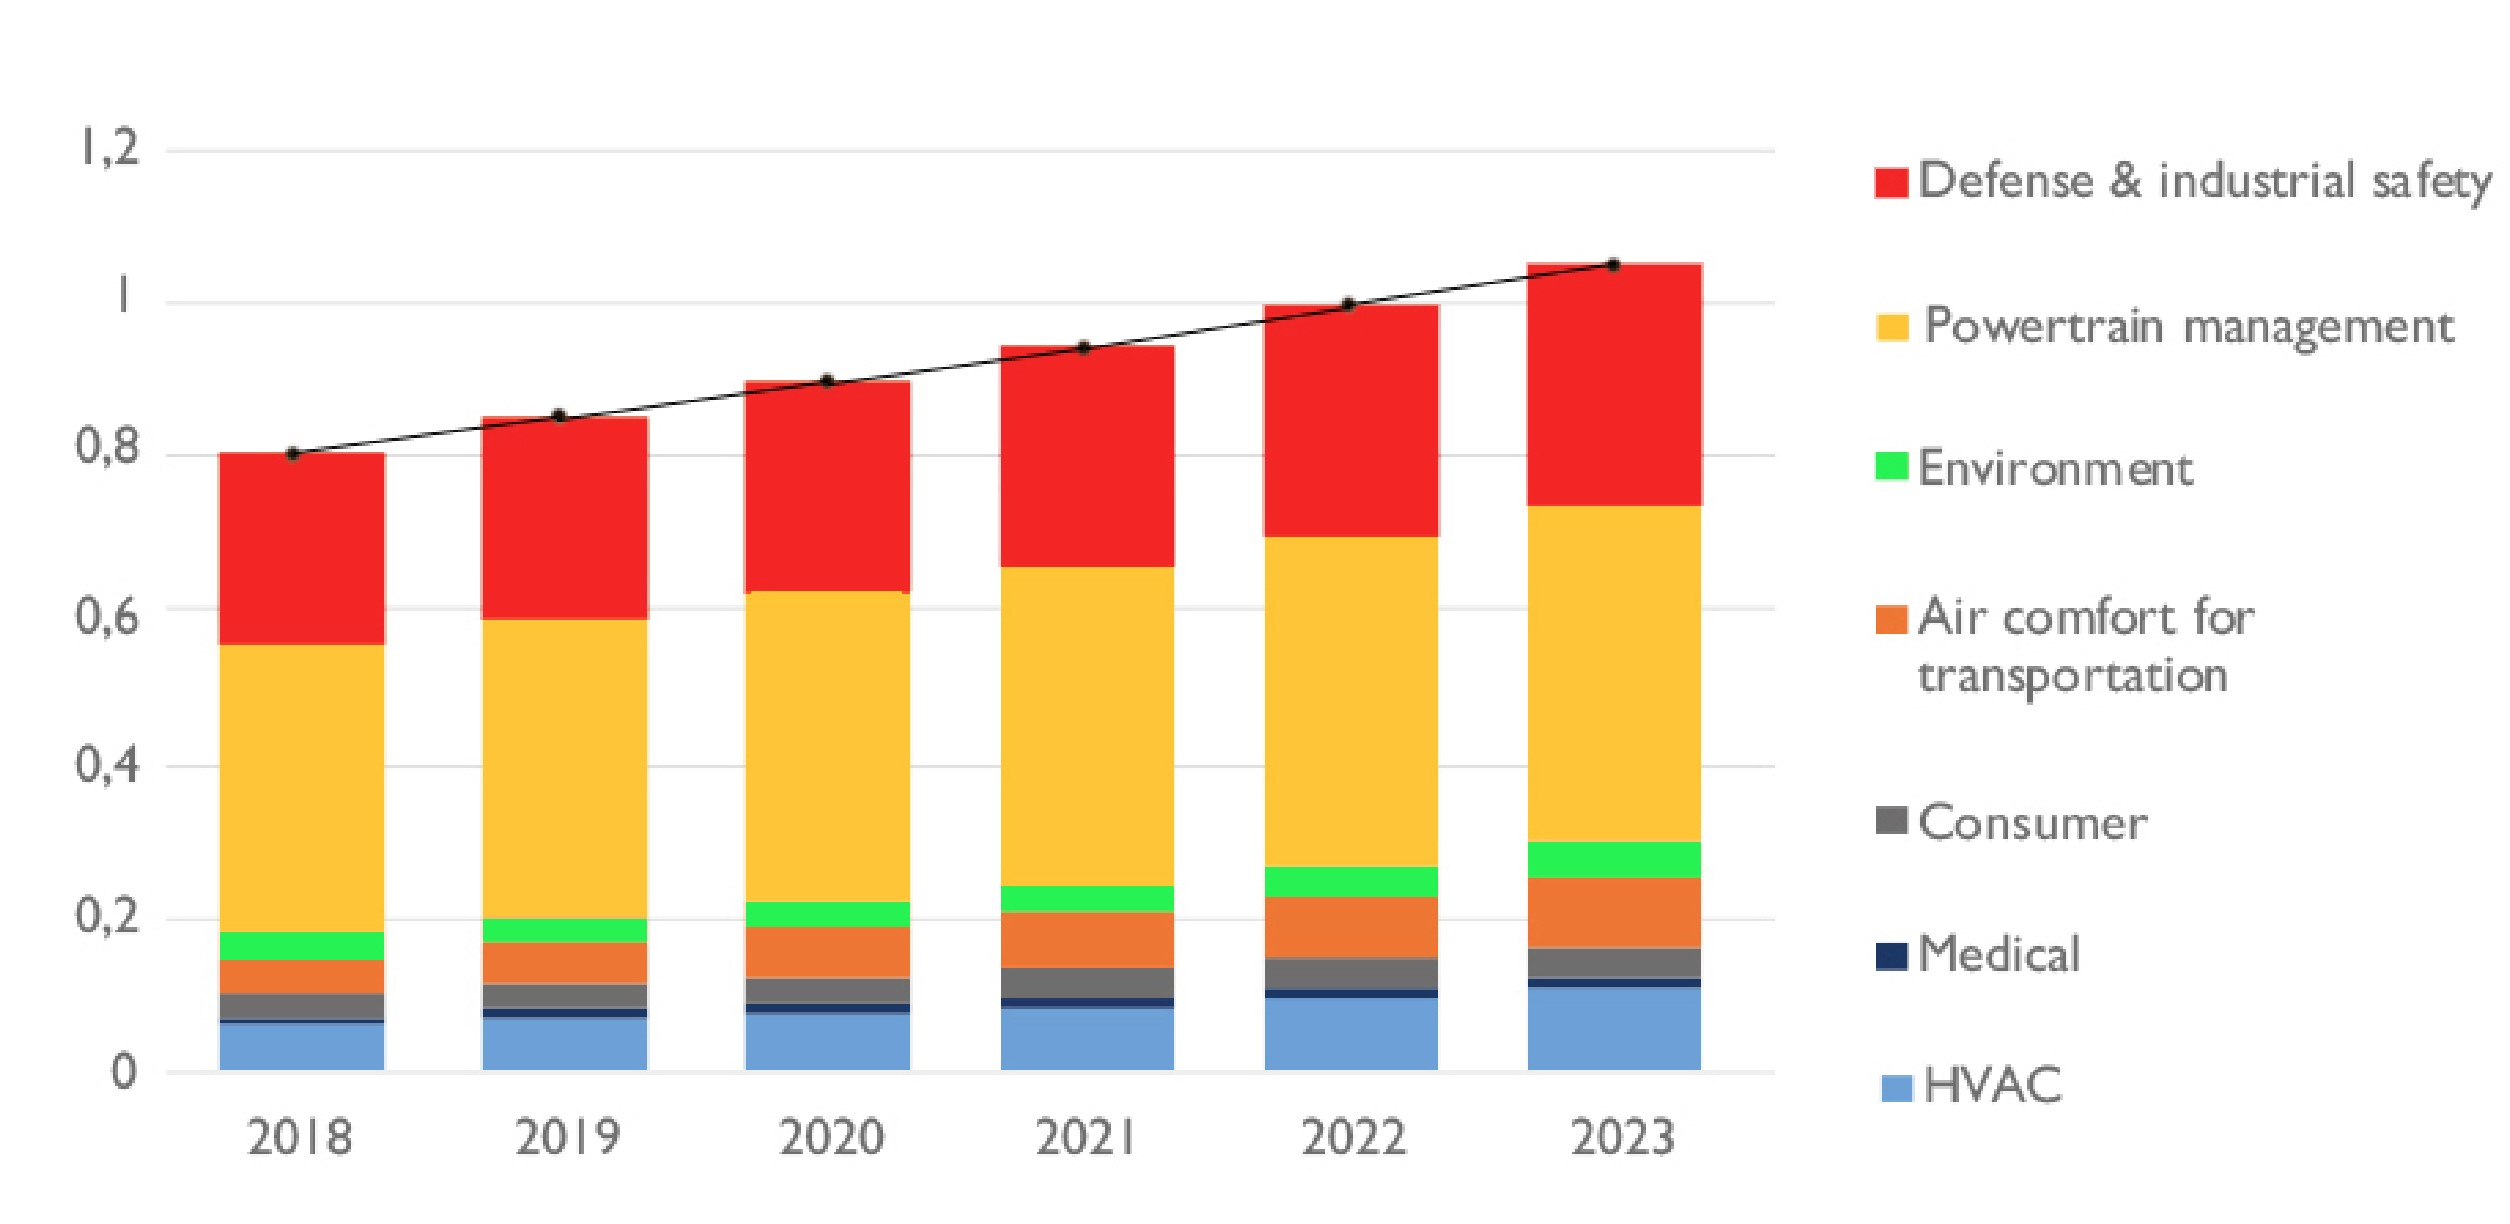
\includegraphics[draft=true]{01_Introduction/fig/gas_sensor_market}
    \caption{The market situation of gas sensors}
    \label{fig:gas_sensor_market}
\end{figure}
Great scientific efforts have been undertaken to find new sensing principles that allow further miniaturization and lowering of the power consumption of the sensors. In the XXXXs, ample expectations have been made to graphene-based sensors. Scientists believed, that the extreme surface to volume ratio favors a higher sensitivity to gases. Ultimately this assumption could not be satisfied. One of the major reasons was the lacking band gap of the material. However, progressing fabrication methods allowed the efficient production of other 2D structures, which which showed the properties, that have been desired from graphene. Holden proposed a sensor based on oxygen and air that provided a sensitivity of very nice and a relaxation time of very short. Albert Einstein tried a different approach with the material combination caliumjodid and fancenstein and achieved a sensitivity of YYY.
These two examples shall testify, that remarkable effects can be shown with 2D structures. One of the most promising material systems are \glspl{tmd}. They show strong sensitivity to gas exposure, have and acceptable recovery time. However, one of its most intriguing properties is the potential compatibility to \gls{cmos} fabrication processes. This feature enables the integration of the sensor onto the same silicon wafer as the digital processor. Thsi processor would then be able to analyze the data generated by the sensor, which enables a highly integrated gas sensing solution.
Due to these fascinating promises, this publication shall shine a light on gas sensor based on 2D \gls{tmd} structures. \Cref{sec:functionality} explains the workings of 2D \glspl{tmd}. After that, the current fabrication methods are layed out in \cref{sec:fabrication}. In order to give an overview above the tunable parameters of 2D \glspl{tmd}, in \cref{sec:2d_tmd_heterojunction_gas_sensors} two different sensor implementations are compared and discussed. Eventually, a summary and outlook is given in \cref{sec:conclusion}.
}